% Numerical data: frozen V29 49-row JSON SHA 0e7bfdb73970fcff9231a51954bd2d548f472cb296624967afc80d9d241ce2be.
\begin{figure}[tb]
\centering
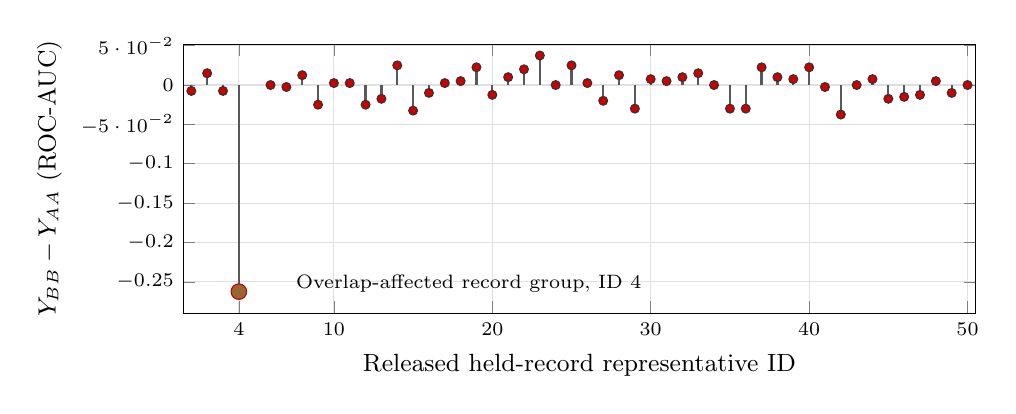
\begin{tikzpicture}
\begin{axis}[
 width=.96\linewidth,height=5.0cm,
 xmin=.5,xmax=50.5,ymin=-.29,ymax=.052,
 xtick={4,10,20,30,40,50},
 ytick={-.25,-.20,-.15,-.10,-.05,0,.05},
 xlabel={Released held-record representative ID},
 ylabel={$Y_{BB}-Y_{AA}$ (ROC-AUC)},
 grid=major,grid style={black!12},
 tick label style={font=\scriptsize},
 label style={font=\small},
 clip=false,
 ]
\addplot+[ycomb,no marks,thick,black!65]
 coordinates {(1,-0.0075) (2,0.0150) (3,-0.0075) (4,-0.2625) (6,0.0000) (7,-0.0025) (8,0.0125) (9,-0.0250) (10,0.0025) (11,0.0025) (12,-0.0250) (13,-0.0175) (14,0.0250) (15,-0.0325) (16,-0.0100) (17,0.0025) (18,0.0050) (19,0.0225) (20,-0.0125) (21,0.0100) (22,0.0200) (23,0.0375) (24,0.0000) (25,0.0250) (26,0.0025) (27,-0.0200) (28,0.0125) (29,-0.0300) (30,0.0075) (31,0.0050) (32,0.0100) (33,0.0150) (34,0.0000) (35,-0.0300) (36,-0.0300) (37,0.0225) (38,0.0100) (39,0.0075) (40,0.0225) (41,-0.0025) (42,-0.0375) (43,0.0000) (44,0.0075) (45,-0.0175) (46,-0.0150) (47,-0.0125) (48,0.0050) (49,-0.0100) (50,0.0000)};
\addplot+[only marks,mark=*,mark size=1.6pt,black!80]
 coordinates {(1,-0.0075) (2,0.0150) (3,-0.0075) (4,-0.2625) (6,0.0000) (7,-0.0025) (8,0.0125) (9,-0.0250) (10,0.0025) (11,0.0025) (12,-0.0250) (13,-0.0175) (14,0.0250) (15,-0.0325) (16,-0.0100) (17,0.0025) (18,0.0050) (19,0.0225) (20,-0.0125) (21,0.0100) (22,0.0200) (23,0.0375) (24,0.0000) (25,0.0250) (26,0.0025) (27,-0.0200) (28,0.0125) (29,-0.0300) (30,0.0075) (31,0.0050) (32,0.0100) (33,0.0150) (34,0.0000) (35,-0.0300) (36,-0.0300) (37,0.0225) (38,0.0100) (39,0.0075) (40,0.0225) (41,-0.0025) (42,-0.0375) (43,0.0000) (44,0.0075) (45,-0.0175) (46,-0.0150) (47,-0.0125) (48,0.0050) (49,-0.0100) (50,0.0000)};
\addplot+[only marks,mark=*,mark size=2.8pt,red!75!black]
 coordinates {(4,-0.2625)};
\node[anchor=west,font=\scriptsize] at (axis cs:7,-.252) {Overlap-affected record group, ID 4};
\end{axis}
\end{tikzpicture}
\caption{Real frozen 49-group paired full-change AUC values
under the original source-macro selection policy. The
single content-overlap-affected group (red marker)
shows a large local decrease after full content-disjoint
source refitting, whereas the other 48 groups have
mixed small gains/losses and a nearly zero average.
Each point is a \emph{processed content group}, not
an independently trained EEG model or a verified unique patient.
The plotted responses are previously exposed outcomes;
no new held target recordings or causal intervention
were introduced for this figure.}
\label{fig:p2-paired-49-localisation}
\end{figure}
